\chapter{混部场景导向的调度定制}\label{chap:sched_policy}

% 本章首先进行内核调度配置的定制,考虑网络敏感型应用要求内核调度以实时性为先,而离线CPU敏感型应用则要求内核调度以吞吐量为先,针对这两种需求设计了响应度优先与吞吐量优先两种内核调度配置。

% 对于CPU资源的隔离,常见的方式是显示地隔离不同应用能够使用的CPU,这种静态的划分方式并不能有效的使用资源,而在本章中提出了基于BPF调度器的调度队列隔离,高低优先级的应用在调度队列优先级机制之上共享相同CPU,使得高优先级应用运行时总是能够优先地使用CPU资源。

% 其次,相较于常见的调度类隔离,本章基于BPF调度器实现更为灵活,通过结合eBPF强大的监测能力,让BPF调度器感知高优先级应用CPU资源、网络资源的使用,而通过设置相关的资源约束,从而结合不同高优先级应用的资源使用特征与调度目标,更充分的利用资源。

为解决不同混部场景下任务调度机制的不足,本章主要展开混部场景导向的定制任务调度机制研究。首先,从内核任务调度的相关配置上,针对不同应用的需求,设计了响应度优先与吞吐量优先两种基础内核配置,随后,在Ext调度类的基础上研究场景导向的BPF Scheduler定制,设计了基于调度队列隔离的QoS保障策略,并在此基础上,结合eBPF的监测能力,进一步设计了CPU资源感知与网络资源感知的任务调度策略。

\section{内核调度配置定制}

Linux调度子系统在设计时力图覆盖足够广泛的场景,但同时也提供了一些编译配置选项,用以针对场景进行优化,这些配置选项围绕时钟与抢占模型的设置展开。

时钟与Linux调度子系统密切相关,在第二章论述中提到,时钟中断是驱动Linux抢占式调度的核心机制,中断的频率决定了调度滴答的周期,而更高的时钟中断频率意味着系统的整体响应度越好。针对时钟中断,内核主要提供了两方面的配置,如表~\ref{tab:config_hz}所示,其中最直接的就是时钟中断的频率配置,内核提供了从100、250、300到1000四种不同的中断频率配置,以满足不同的场景下对于响应度的需求,而值得注意的是,由于内核在每个时钟中断处理中进行时间记账,并将两次时钟中断所间隔的时间片累计到当前进程的记账中,然而在实际情况下两次时钟中断中间很有可能夹杂了其他任务的处理,所以更高的时钟中断频率不仅能带来响应度的提升,还能够增强任务时间记账的准确性。其次,考虑到时钟中断会引入额外的计算开销,而在一些场景中这些开销是非必要的,如当CPU进入Idle状态,此时处理时钟中断不仅没有意义,还会增加系统的开销,因此内核提供了NO\_HZ相关配置来在特定场景下屏蔽时钟中断。

\begin{table}
    \bicaption{\quad 内核时钟中断配置}{\quad Kernel Clock Interrupt Configuration}% caption
    \label{tab:config_hz}
    \footnotesize% fontsize
    \setlength{\tabcolsep}{4pt}% column separation
    \renewcommand{\arraystretch}{1.5}% row space 
    \centering
    \begin{tabular}{lc}
        \hline
        配置名称 & 描述 \\
        \hline
        HZ\_100  & 配置时钟中断频率为100  \\
        HZ\_250  & 配置时钟中断频率为250 \\
        HZ\_300  & 配置时钟中断频率为300 \\
        HZ\_1000 & 配置时钟中断频率为1000 \\
        HZ\_PERIODIC & 永远不要忽略时钟中断 \\
        NO\_HZ\_IDLE & 忽略空闲CPU上的时钟中断 \\
        NO\_HZ\_FULL & 忽略空闲CPU,以及只有一个可运行任务CPU上的时钟中断 \\
        \hline
    \end{tabular}
\end{table}

抢占指执行任务时,允许高优先级的任务打断低优先级任务的执行,从而提供更好的响应度。用户态任务的执行总是能够被打断,而内核态任务的抢占则较为复杂,为此内核提供了抢占模型的编译配置,允许用户针对不同场景进行调整,相关配置如表~\ref{tab:config_preempt}所示, 内核提供了PREEMPT\_NONE、PREEMPT\_VOLUNTARY、PREEMPT以及PREEMPT\_RT四种抢占模式,四种模式下内核的响应度逐步增强。

\begin{table}
    \bicaption{\quad 内核抢占模式配置}{\quad Kernel Preemption Configuration}% caption
    \label{tab:config_preempt}
    \footnotesize% fontsize
    \setlength{\tabcolsep}{4pt}% column separation
    \renewcommand{\arraystretch}{1.5}% row space 
    \centering
    \begin{tabular}{lc}
        \hline
        配置名称 & 描述 \\
        \hline
        PREEMPT\_NONE  & 内核代码保持执行直到主动放弃CPU  \\
        PREEMPT\_VOLUNTARY  & 开启了内核代码中的抢占位点 \\
        PREEMPT  & 提供更多的内核代码抢占位点,实现完全抢占 \\
        PREEMPT\_RT & 进一步修改内核代码的实现,如锁机制,实现实时可抢占性 \\
        \hline
    \end{tabular}
\end{table}

时钟和抢占模式的配置能够决定系统的响应度,但实际的配置需要考虑使用的场景,如更高的HZ虽然能够提升系统的整体响应度,但由于时钟中断的增多,CPU在于有限的时间片内处理实际任务的时间就会变少,同时频繁的上下文切换也破坏了程序的时间局部性,从而影响到系统的整体吞吐。通常而言,较高的HZ与激进的抢占模式有利于降低延时,而较低的HZ与保守的抢占模式有利于系统的整体吞吐。对此Control Zone提供了两种预编译的内核,用于处理响应度优先与吞吐量优先两种场景。

\section{资源感知的任务调度}

% Control Zone内调度
% - 互斥调度:用于SMT或保守调度策略
% - 有资源阈值的互斥调度: 资源达到阈值时,才进行互斥调度(系统资源达到阈值时,使能BPF Scheduler)
%   - Memory、CPU、Network、IO

\subsection{调度队列隔离策略}

% Linux Fair调度队列问题
% - 单个CPU上的任务同属于一个调度队列
% - 优先级机制用于限制不同任务对CPU时间的使用,并不能保证高优先级的应用一定能够比低优先级应用优先调度
% 使用实时调度类与Idle调度类存在的问题
% - 运行在实时调度类中的LC任务如配置不当,一方面不利于应用性能,另一方面容易造成系统崩溃
% - 将低优先级的任务允许在Idle类是嵌入式领域的常用做法,但不够灵活,且违背Linux设计语义

多任务调度场景可分为两种。第一种是单CPU调度队列上的任务调度,此时任务分时复用CPU资源,调度策略通常采用优先级机制,并优先为高优先级任务分配CPU时间。第二种则是多CPU调度队列上的任务调度,Linux内核在这种场景下通常会允许任务在一定程度上的并发, 同时利用负载均衡机制来避免任务过度集中。

混部场景下,声明静态优先级来指示操作系统优先为高优先级任务提高资源是常见的手段。然而这种方式存在一些问题,对于默认的Fair调度类,在第二章的分析中,CFS调度器会减缓高优先级任务的vruntime积累,使得高优先级任务更容易被调度,但是这种方式是尽力而为的,随高优先级任务占用越来越多的CPU时间,其优先级就会被不断削弱直至被低优先级任务抢占。造成这种现象的根本原因是混部应用处在相同的调度队列中,而多数调度器的设计中都会尽量避免队列中的任务出现饥饿,但在混部场景中,对于LC任务而言这种需求是确实存在的。

另一种方式则是利用调度类的优先级差异将混部应用放置到不同的调度类中,从而实现调度队列的隔离性,但这种方式也存在一些缺陷,首先,选择将高优先级应用放置在实时调度类中,一方面需要针对性地配置调度类选项,如Deadline调度器的runtime、period、deadline参数,以适应高优先级的运行特征,另一方面设置实时调度类并非是安全的操作,需要谨慎地处理优先级配置以避免抢占如softirq等重要内核线程,导致系统运行受到影响。其次,选择将低优先级任务放置到Idle调度类中,这在嵌入式等资源受限场景下较常使用,但是这种方式不够灵活,且违背了Linux Idle调度类的设计语义,容易造成资源浪费与性能下降。

而使用BPF Scheduler则可以解决如上问题。首先,Ext调度类介于Fair调度类与Idle调度类之间,一方面提供了隔离的调度队列,另一方面也避免了与现有的调度类中任务的冲突。本研究基于BPF Scheduler提供了三种基本调度策略:

1)基于FIFO的非抢占式调度:BPF Scheduler中使用FIFO DSQ(分发队列),并设置每个入队任务的时间片为无限,任务运行直到主动退出,随后BPF Scheduler取出下一个任务执行。

2)基于RR的抢占式调度:BPF Scheduler中使用FIFO DSQ, 并按照配置设置每个入队任务的时间片,每次时钟滴答时检查当前任务的剩余时间片,抢占时间片耗尽的任务并切换到下一个任务执行。

3)基于vtime的抢占式调度:BPF Scheduler中使用vtime DSQ,vtime DSQ按照vtime大小对任务进行排序,初始时设置每个入队任务的初始vtime,并在每个时钟滴答里根据任务的静态优先级更新vtime,抢占发生时,vtime越小的任务越优先被调度。

混部场景中的LC应用多由网络驱动,而结合第二章中对于调度循环的分析,使能调度队列隔离策略之后,每当网络中断处理完毕时,处在更高优先级队列中的LC应用必然会优先于BE应用被调度,同时在LC应用的运行过程中,处在相同CPU上的BE应用也不会抢占LC应用,从而能够在任务调度的角度最大限度地保障LC应用的QoS。

调度队列隔离策略实质上提供了低优先级任务感知高优先级任务运行的基本机制,而在此基础上,可以结合其他资源约束条件,来进一步地强化隔离,从而更好地来保障应用QoS,或者在一定条件下允许部分地并发,来提升资源利用率。

\subsection{CPU资源感知策略}

% 与 Core Scheduler的区别
% - Core Schedule使用固定的CPU拓扑
% - Bpf Schedule可自由定义CPU Cgroup

Linux采用调度域机制来描述不同的CPU特性,而在第一章的分析中提到,由于SMT、NUMA、CPU Turbo等技术的存在,独立的CPU之间仍然存在资源的竞争,这就导致了混部场景下的吵闹邻居现象。单一调度队列中,优先级机制能够指示任务的调度行为,但在不同CPU调度队列上,优先级机就几乎不能产生影响,如在一个SMT系统中,即便运行在不同Sibling上的任务存在优先级差异,但此时调度器并不能保证高优先级任务的资源使用。

对于CPU敏感型应用,如上问题会引发较大的性能劣化,为此本研究进一步设计了CPU资源感知策略。策略允许低优先级任务的调度的CPU阈值,允许当低优先级任务的可用CPU数量达到阈值时,才能进行任务调度,否则则需要让出CPU资源。相较于Linux Core调度,CPU资源感知策略不局限于SMT编组,提供更灵活的调度方案。而相较于Cgroup中的cpu set机制,CPU资源感知策略使用更动态的CPU数量而不是固定的CPU亲和性,从而能够实现高优先级任务空闲时,利用所有的空闲核心,而当高优先级任务运行时,来根据阈值控制并发数量。

\begin{algorithm}
    \caption{Pseudocode for Enhanced Task Scheduling Isolation Mechanism}
    \label{alg:cpu_aware_sched}
    \begin{algorithmic}[1]
    
    \Function{cpuAcquire} {cpu}
    \State Insert cpu to CPU\_Map;
    \EndFunction
    
    \Function{cpuRelease} {cpu}
    \State Remove cpu from CPU\_Map;
    \EndFunction
    
    \Function {schedule}{}
        \While{True}
            \If{$\text{CPU\_Acquired + CPU\_Idle} < \text{CPU\_Available}$ }
                \State Set Exclusive Flag;
                \For{each no\_hz core C}
                    \State Send an IPI to envoke target CPU rescheduling.
                \EndFor
                \State Yield to higher priority scheduler class;
            \EndIf
            \State Remove Exclusive Flag;
            \State Dispatched tasks;
        \EndWhile
    \EndFunction
    \end{algorithmic}
\end{algorithm}

而在实际BPF Scheduler中,选择使用一个全局DSQ,并通过cpu\_acquire,cpu\_release两个回调函数来动态获取当前Ext调度类中所能管理的CPU数量,而具体的调度逻辑如伪代码~\ref{alg:cpu_aware_sched}所示,首先BPF Scheduler会依据不同调度类CPU的数量,来判断是否有更高优先级调度类中的任务正在运行,一旦发现,则首先设置一个Exclusive Flag, 用于在其他回调中共享状态,其次,对于处于NoHZ状态下的CPU,发送IPI以注入一次重调度,而当系统中没有更高优先级调度类的任务运行时,则正常进行任务的分发。

\subsection{网络资源感知策略}

% LC应用负载与Epoll的关系
% - 原理
% - 流量,epoll wait图,相关性
% 网络资源感知策略

网络资源敏感型应用的构成中并非所有部分都与网络相关,如Redis主线程监听网络请求并进行处理,而用于快照的辅助线程则与网络无关,同时,在第三章的应用画像中也发现网络资源敏感型应用的资源敏感度随负载而变化。以上都使得网络资源的使用情况能够作为一种进行调度决策的因素。

大多数高性能网络应用都基于epoll机制实现。epoll机制允许进程同时监听多个连接,并在连接就绪时进行批量处理,相较于阻塞型网络系统调用,使用epoll能够在大量请求时减少频繁地阻塞唤醒过程,从而支持更高的并发量。epoll机制涉及到多个系统调用,而其中最为核心的是epoll\_wait系统调用,进程在注册等待事件之后,就能够通过epoll\_wait系统调用来获取当前的就绪事件,当存在就绪事件时,epoll\_wait系统调用会返回就绪的事件数量,而当没有事件就绪时,epoll\_wait仍然会阻塞进程。

\begin{figure}[H]
    \centering
    \begin{subfigure}[b]{0.49\textwidth}
        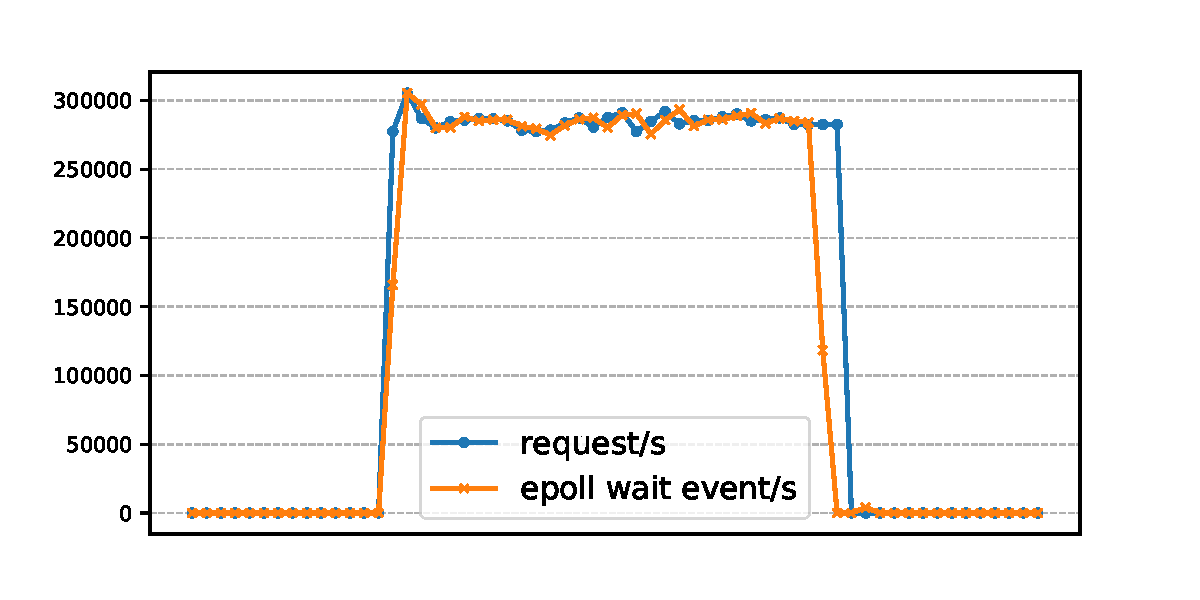
\includegraphics[width=\textwidth]{epoll_memcached}
        \caption{Memcached请求数量与Epoll Wait事件数量}
        \label{fig:epoll_memcached}
    \end{subfigure}
    \begin{subfigure}[b]{0.49\textwidth}
        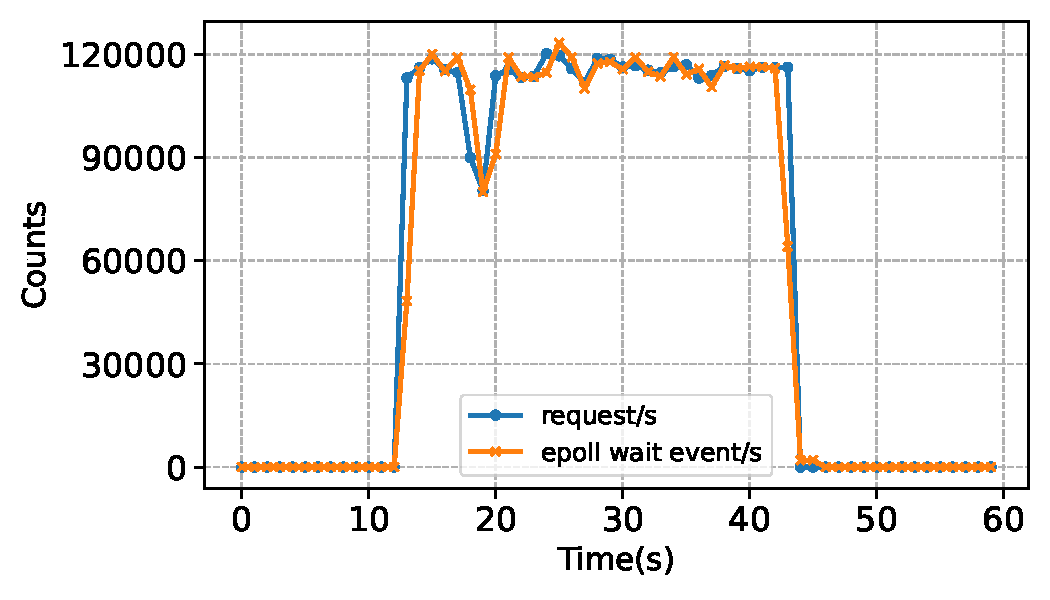
\includegraphics[width=\textwidth]{epoll_redis}
        \caption{Redis请求数量与Epoll Wait事件数量}
        \label{fig:epoll_redis}
    \end{subfigure}
\bicaption{\quad LC应用负载与Epoll事件}{\quad Requests and Epoll Events on LC}
\label{fig:epoll_request}
\end{figure}

综合以上分析,网络资源的使用监测可通过监听epoll\_wait系统调用的执行以及其返回参数实现,而使用eBPF技术能够方便地对系统调用进行探测。结合第三章中的eBPF系统调用探测的实现,网络资源监听eBPF程序在epoll\_wait返回处进行插桩,并统计epoll\_wait的执行频率与总事件计数,其次,eBPF程序额外记录了当次epoll\_wait完成的时间戳及事件数量,用以捕获突发的事件。截取Redis与Memcached在工作负载下的指标序列,绘制如图~\ref{fig:epoll_request}所示的折线图,能够分析,对于Redis与Memcached这两类典型的网络应用,epoll\_wait事件数量与请求数量高度相关,由于实验中由于请求计量在client侧,epoll\_wait事件计数则在server侧,因此两段序列会存在一定的偏移。

eBPF程序之间的数据能够方便地通过BPF Map共享,而基于对于epoll wait的探测程序实现的网络资源感知BPF Scheduler具体逻辑如伪代码~\ref{alg:network_aware_sched}所示。在BPF Scheduler在获取到CPU的管理权限之后,还需要根据当前系统中的网络资源使用情况来判断是否进行低优先级任务的调度,网络资源的阈值可以结合第三章中的无干扰画像进行灵活的配置,主要在低负载段允许任务的并发以充分利用系统资源。

\begin{algorithm}[H]
    \caption{Pseudocode for Network Resource Constraints Scheduling Strategy}
    \label{alg:network_aware_sched}
    \begin{algorithmic}[1]

    \Function {do\_epoll\_wait\_return}{$nr\_event$}
        \State Write timestamp of current epoll wait;
        \State Write $nr\_event$ of current epoll wait;
        \State Update total event count;
        \State Update count of epoll wait;
    \EndFunction

    \Function {schedule}{}
        \While{True}
            \State Read epoll wait delta from bpf map;
            \If{$\text{EPOLL\_WAIT\_DELTA} < \text{EPOLL\_WAIT\_THRESHOLD}$ }
                \State Set Exclusive Flag;
                \For{each no\_hz core C}
                    \State Send an IPI to envoke a rescheduling;
                \EndFor
                \State Yield to higher priority scheduler class;
            \EndIf
            \State Remove Exclusive Flag;
            \State Dispatched tasks;
        \EndWhile
    \EndFunction
    \end{algorithmic}
\end{algorithm}

基于调度队列的隔离会在高优先级任务执行时进行避让,因此BPF Scheduler网络资源感知策略仍然相对保守,导致无法充分地使用系统资源。对此有两种解决方式,第一种方式是将高优先级应用也加入到Ext调度类中,并单独为其分配一个DSQ,这种方式对BPF Scheduler的实现要求较高。而第二种方式则相对简单,eBPF的优势在于其灵活性,因此上述逻辑也可以变更为在低负载时,关闭BPF Scheduler,而根据第二章的技术分析,此时所有的EXT调度类任务将回退到Fair调度类中,从而解除调度队列隔离,而当负载达到一定阈值时,再使能BPF Scheduler来保障高优先级任务的性能。

% \subsection{基于PMU实现的其他资源感知策略}

\section{实验设计与分析}

\subsection{响应度优先内核性能}

% redis \ memcached

Control Zone响应度优先配置使用HZ\_1000配置时钟中断,并开启PREEMPT抢占模式。响应度优先内核的优势主要体现在多任务调度场景,因此在实验设计上,选择Redis、Memcached两种CPU敏感型应用来分别与CPU干扰应用混部以构造多任务场景,并使用CloudHypervisor默认提供的内核作为基准进行比较。实验在一个4CPU 512MB内存的Control Zone中进行。

\begin{figure}[H]
    \centering
    \begin{subfigure}[b]{0.49\textwidth}
      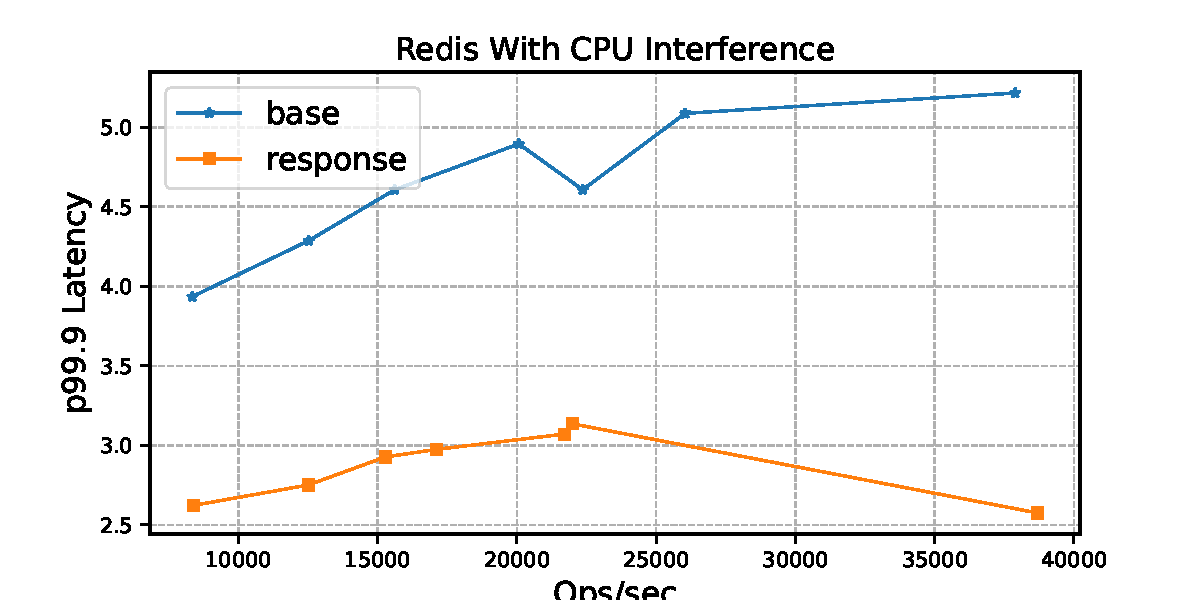
\includegraphics[width=\textwidth]{redis_response}
      \caption{Redis与干扰混部}
      \label{fig:redis_response}
    \end{subfigure}
    \begin{subfigure}[b]{0.49\textwidth}
      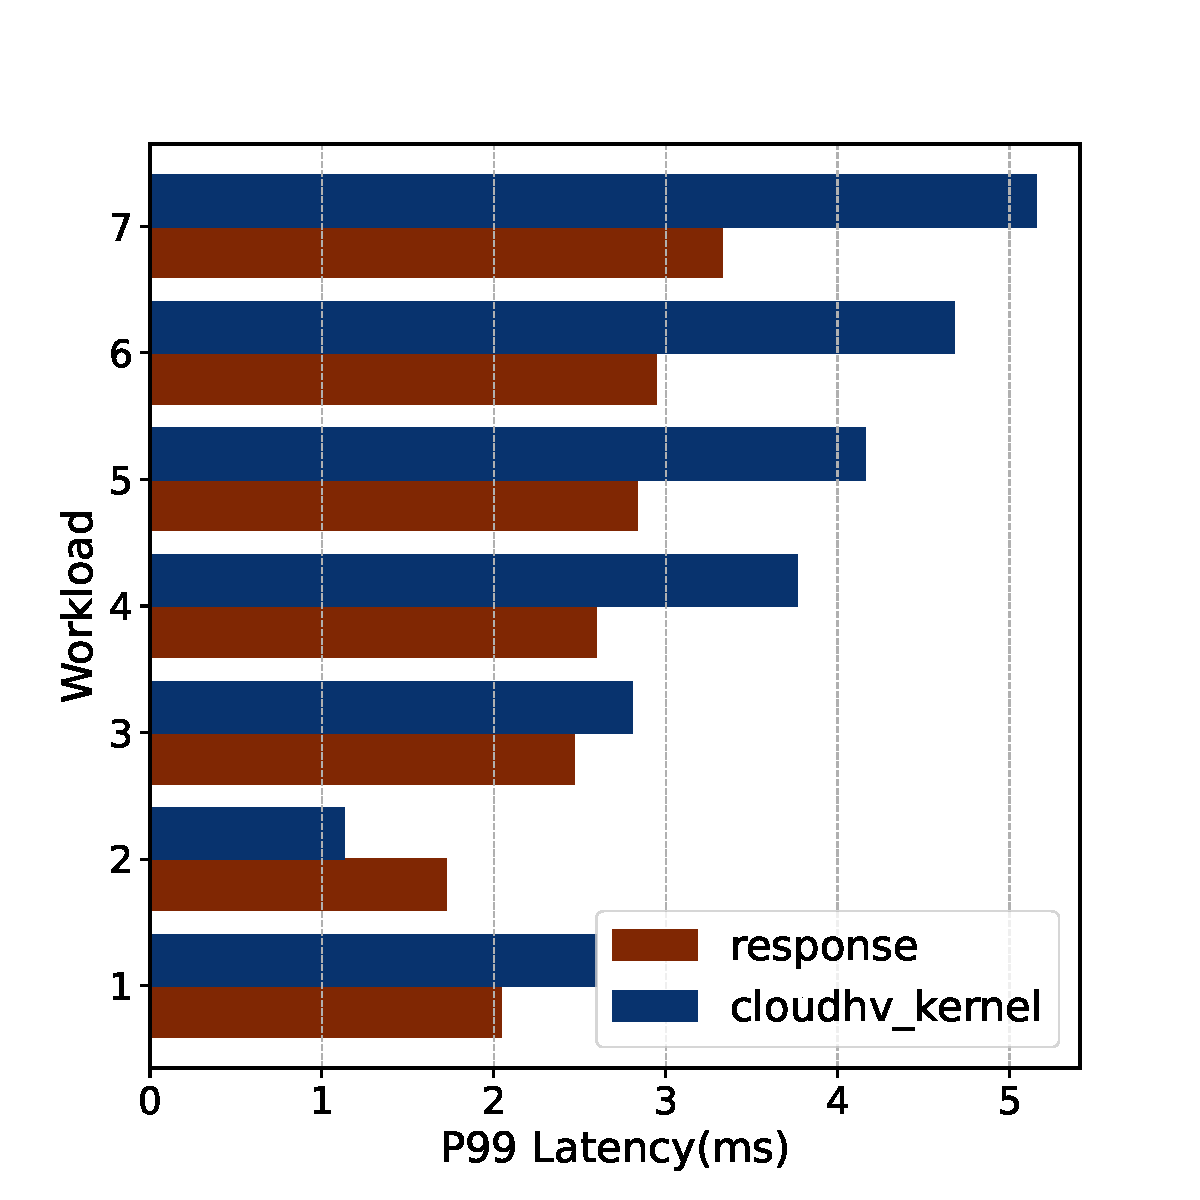
\includegraphics[width=\textwidth]{memcached_response}
      \caption{Memcached与干扰混部}
      \label{fig:memcached_response}
    \end{subfigure}
    \bicaption{\quad 混部场景下的响应度优先内核}{\quad Response Priority Kernel in Mixed Deployment Scenarios}
    \label{fig:lc_response}
\end{figure}

混部实验结果如图~\ref{fig:lc_response}所示,在启用Control Zone响应度优先内核后,无论是Redis还是Memcached,在P99.9延迟上都要优于CloudHypervisor的默认内核,Reponse内核使用了更高的时钟中断频率,因此能够更快地在延时敏感应用与干扰应用中进行切换,同时在PREEMPT抢占模式下,网络中断能够更及时地进行处理,降低请求处理链路的整体延时。

\subsection{吞吐量优先内核性能}

% graph500(time) \ ffmjpeg 

Control Zone吞吐量优先配置使用HZ\_100配置时钟中断,并开启PREEMPT\_NONE抢占模式。吞吐量优先内核能够在任务量较少的场景中,让任务保持CPU资源的占用,从而更好地利用局部性,因此实验使用单一任务场景,选择Graph500作为目标应用,并对比其在CloudHypervisor默认内核、Throughput内核以及Response内核下的运行情况。实验在一个4 CPU、512MB内存的Control Zone中进行。

\begin{figure}[H]
    \centering
    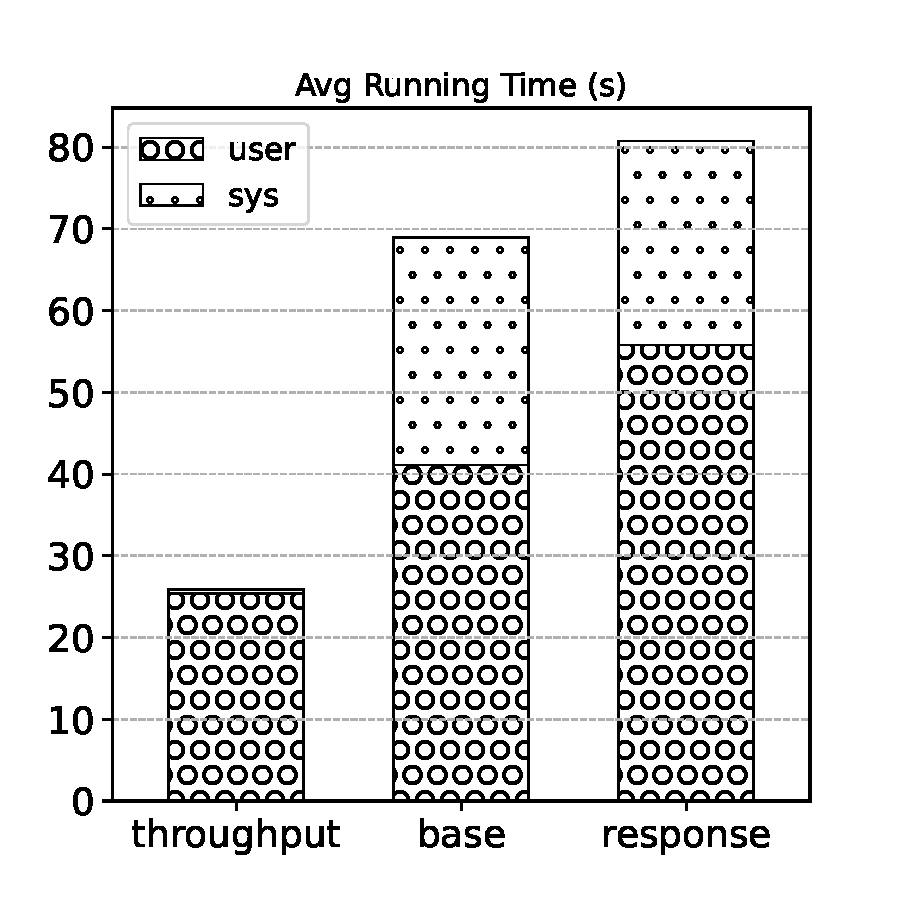
\includegraphics[width=0.5\textwidth]{avg_graph500_runtime}
    \bicaption{\quad 吞吐量优先内核配置优化效果}{\quad Throughput Discrepancy Across Different Configurations} 
    \label{fig:avg_graph500_runtime}
\end{figure}

Graph500主要执行图计算算法,因此执行时间是其重要的性能指标,实验中使用time工具记录任务的执行时间,包括用户态与内核态的执行时间, 具体实验结果如图~\ref{fig:avg_graph500_runtime}所示,其中使用Throughput内核的Control Zone消耗的时间最短,而使用Response内核的Control Zone则消耗的最长的时间,分析执行时间占比,在Throughput内核下,任务运行过程中内核态时间消耗几乎没有,而在Response内核中,内核态时间则占用了较大比例,造成这一结果的主要原因是时钟中断与NO\_HZ配置,越高的时钟中断频率会引发越导致越频繁的陷入内核态,一方面使得内核态时间变得更长,另一方面也会导致局部性的破坏导致任务执行速度的减慢。

\subsection{CPU资源感知策略效果}

% 普通场景
% 硬件场景:SMT

BPF强隔离调度策略能够在混部场景中,为高优先级应用提供更好的性能保障,使得性能接近于无干扰的状态。而为验证强隔离调度策略的效果设计了两个混部场景的实验。场景一中使用4个独立的CPU,2048M内存的Control Zone进行实验,高优先级应用使用Mysql,而低优先级应用使用CPU干扰应用。场景二中则使用2CPU,512M的内存,并特别地使用SMT绑定为虚拟机CPU,同时选用延时敏感的Redis与CPU干扰进行混部。

混部场景一实验结果如图~\ref{fig:mysql_perf}所示,首先能够看出,Linux EEVDF调度器默认下以公平为目标,此时Mysql的性能并不能得到保障,而在降低CPU干扰应用的nice值之后,Mysql的性能虽然有一些提升,但相较于无干扰情况下仍存在较大劣化, 而分析Control Zone CPU使用率能够发现,Mysql在正常运行时并不会占用所有的核心,此时即便与干扰应用存在优先级上的差异,但由于这种优先级并不能跨越CPU调度队列产生效果,因此仍然存在一定程度上的并发,而由于资源竞争的Mysql的性能就会出现劣化。而在启用了BPF调度器之后Mysql性能几乎与没有干扰的情况下一致,首先,尽管优先级机制不能跨越核心产生作用,但在BPF调度器中能够自已强隔离的所里,使得高优先级的Mysql在运行时,低优先级的干扰应用能够自动的让出CPU,从而实现高优先级任务的性能保障。

\begin{figure}[!htbp]
    \centering
    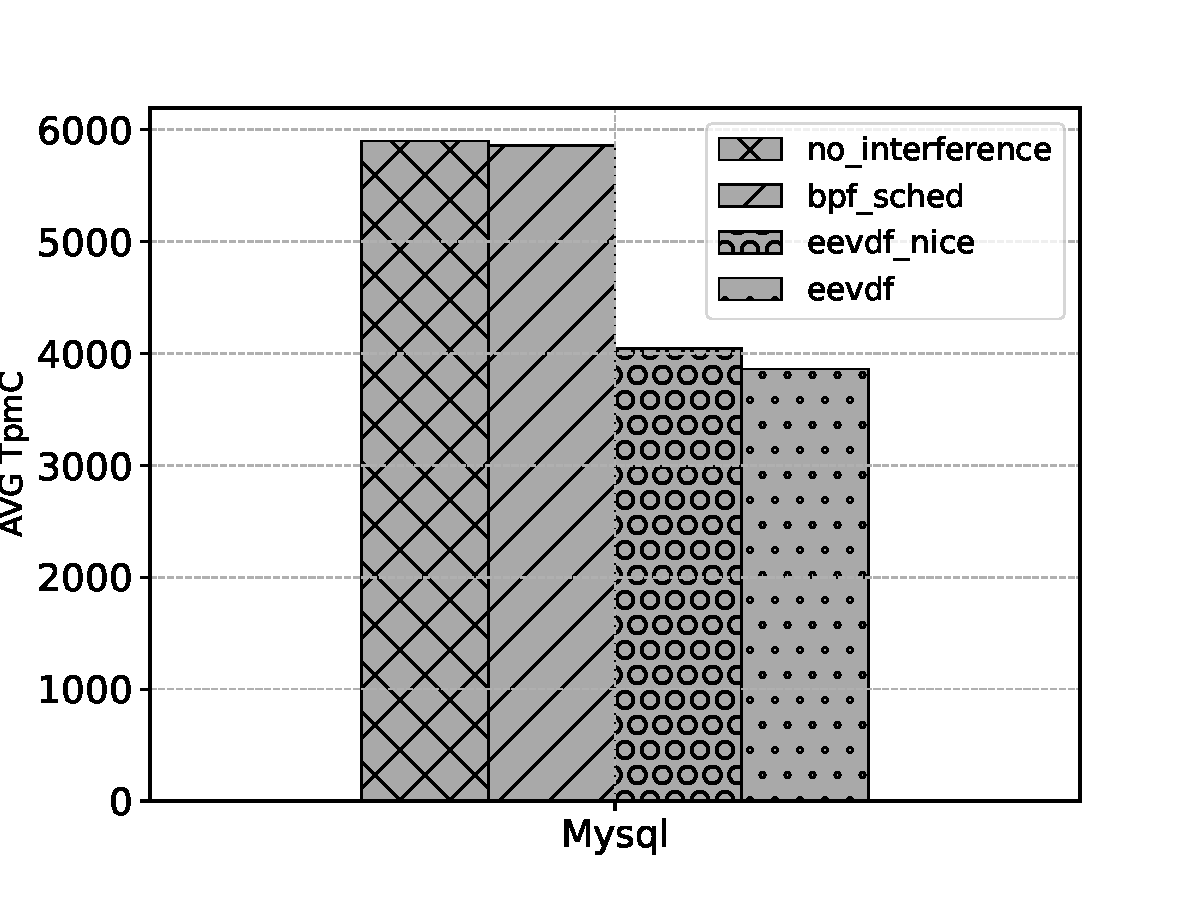
\includegraphics[width=0.6\textwidth]{mysql_perf}
    \bicaption{\quad Mysql与干扰混部}{\quad MySQL with Interference} 
    \label{fig:mysql_perf}
\end{figure}

混部场景二实验结果如图~\ref{fig:redis_smt}所示。SMT下Sibling共享了同一个物理CPU上的片上资源, 因此混部存在更激烈的资源竞争。Elfen\citep{yang2016elfen}通过修改内核与BE应用,使得BE应用能够主动探测Sibling上LC应用并及时出让CPU,从而保障LC应用的性能。这一思路在SMT场景中十分重要,而在BPF CPU感知任务调度策略中,首先,可以在Control Zone的资源声明中标注SMT信息,随后在BPF调度器启动时可以利用此参数,并在调度时考虑Sibling的运行情况。从实验结果中也能够看出,相较于Linux默认调度器,BPF调度器能够在干扰混部的场景中,使得LC应用在低负载时降低79.6\%的延迟,并在高负载时仍有33.7\%的延迟降低效果,这说明BPF Scheduler能够在不同负载下保障LC应用,使其性能接近于无干扰的情况

\begin{figure}[!htbp]
    \centering
    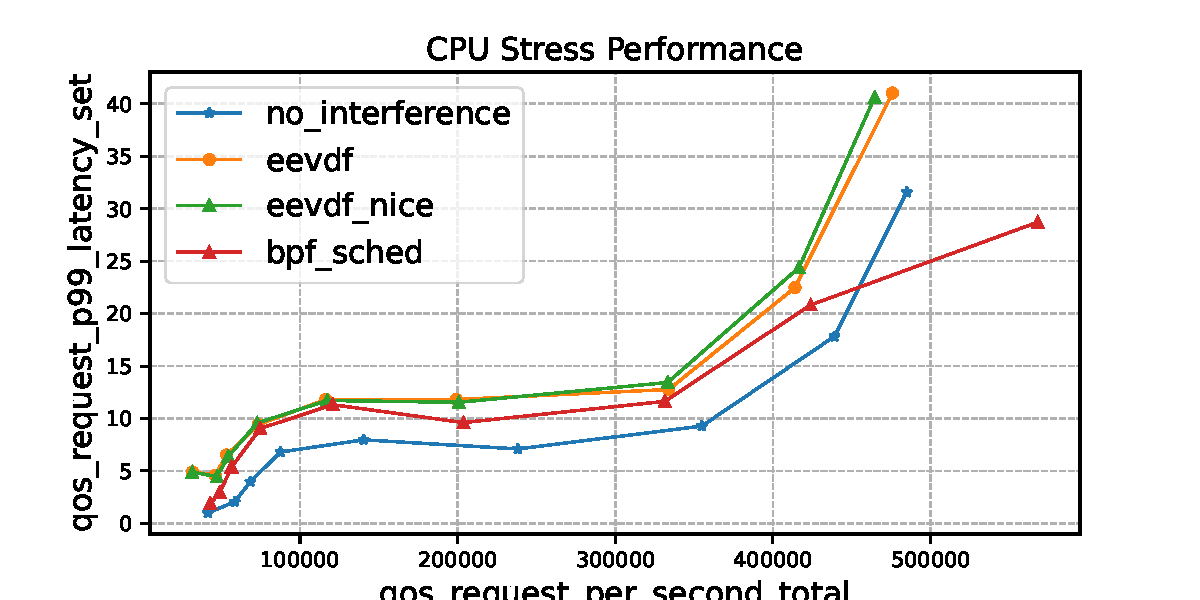
\includegraphics[width=0.6\textwidth]{redis_smt}
    \bicaption{\quad SMT下Redis与干扰混部}{\quad Redis with Interference On SMT} 
    \label{fig:redis_smt}
\end{figure}

\begin{figure}[H]
    \centering
    \begin{subfigure}[b]{0.49\textwidth}
        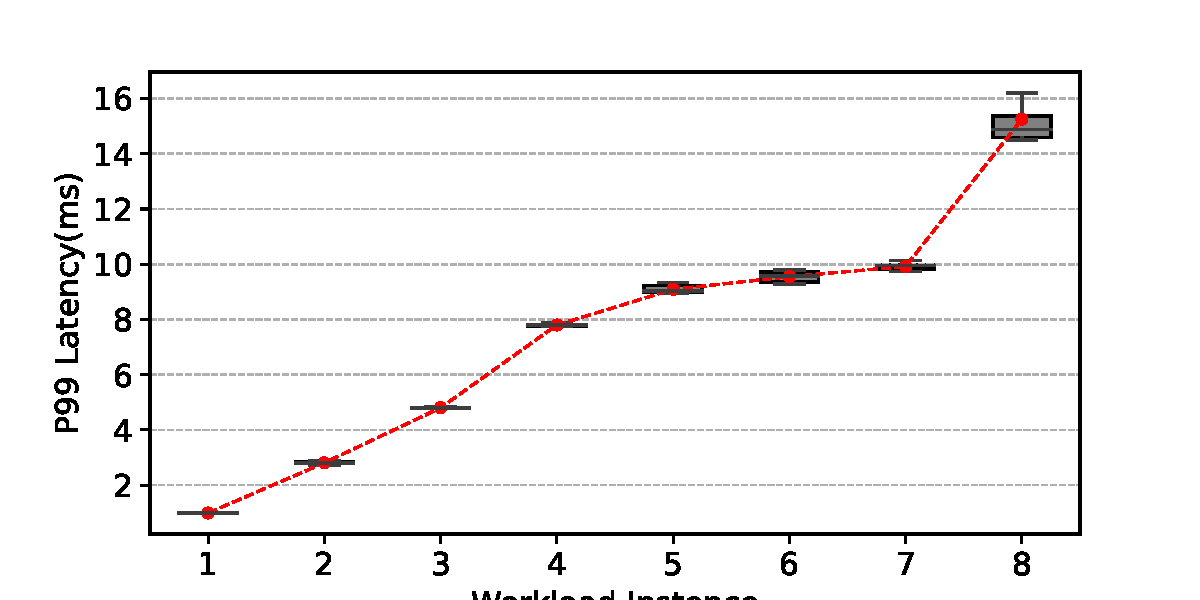
\includegraphics[width=\textwidth]{cpu_aware_box_bpf_sched}
        \caption{无干扰下Redis延迟}
        \label{fig:cpu_aware_box_bpf_sched}
    \end{subfigure}
    \begin{subfigure}[b]{0.49\textwidth}
        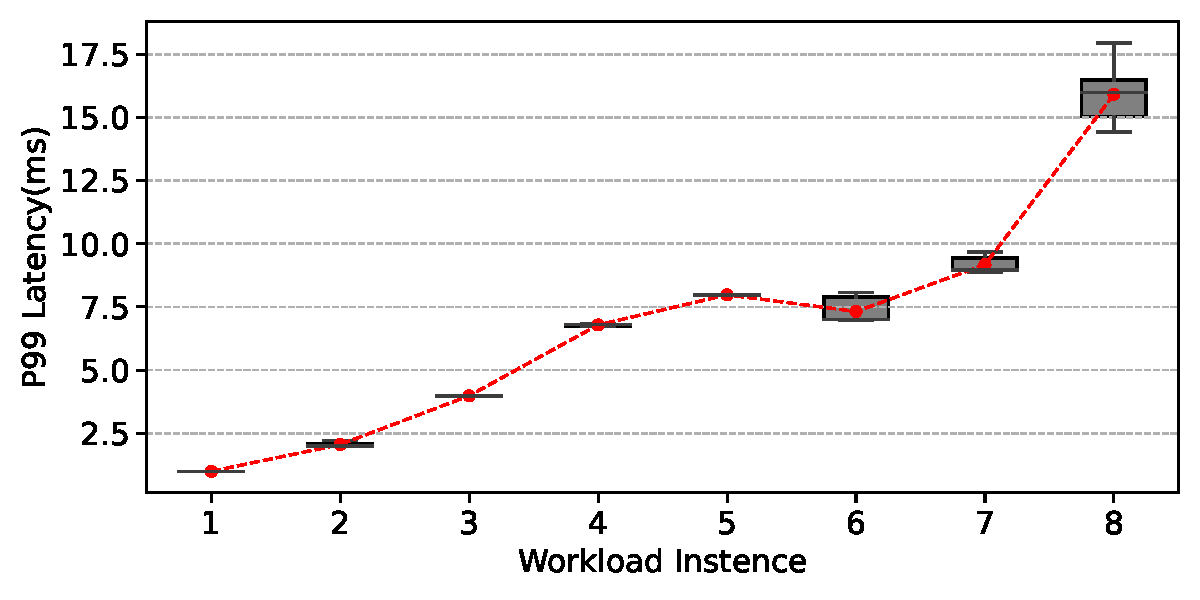
\includegraphics[width=\textwidth]{cpu_aware_box_no_interference}
        \caption{混部场景BPF调度器}
        \label{fig:cpu_aware_box_no_interference}
    \end{subfigure}
    \begin{subfigure}[b]{0.49\textwidth}
        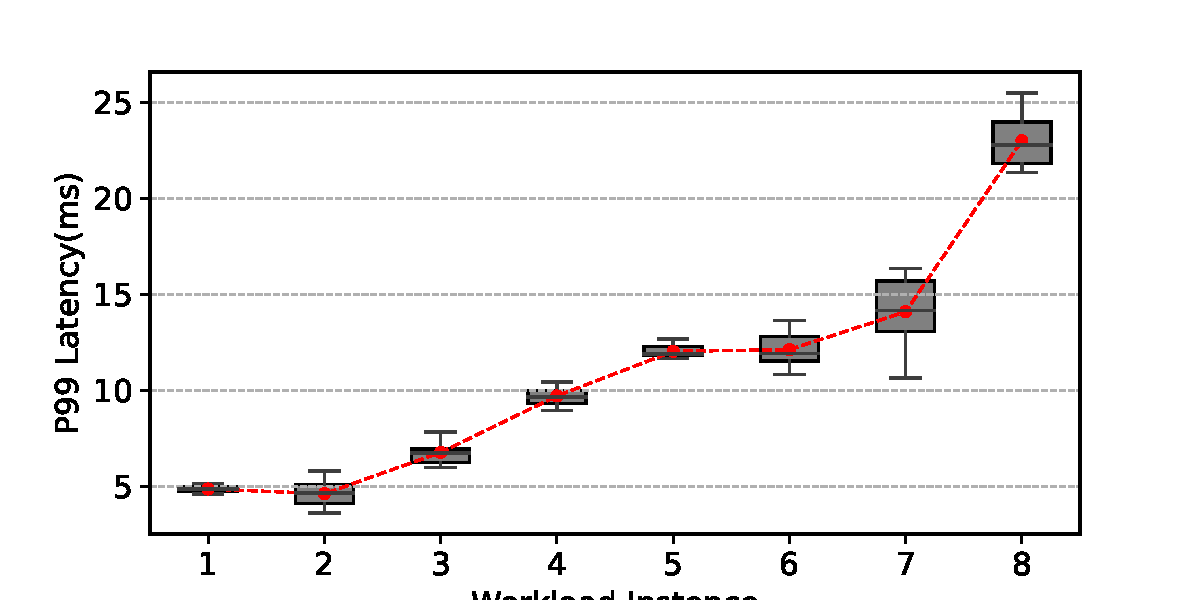
\includegraphics[width=\textwidth]{cpu_aware_box_eevdf}
        \caption{混部场景EEVDF调度器}
        \label{fig:cpu_aware_box_eevdf}
    \end{subfigure}
    \begin{subfigure}[b]{0.49\textwidth}
        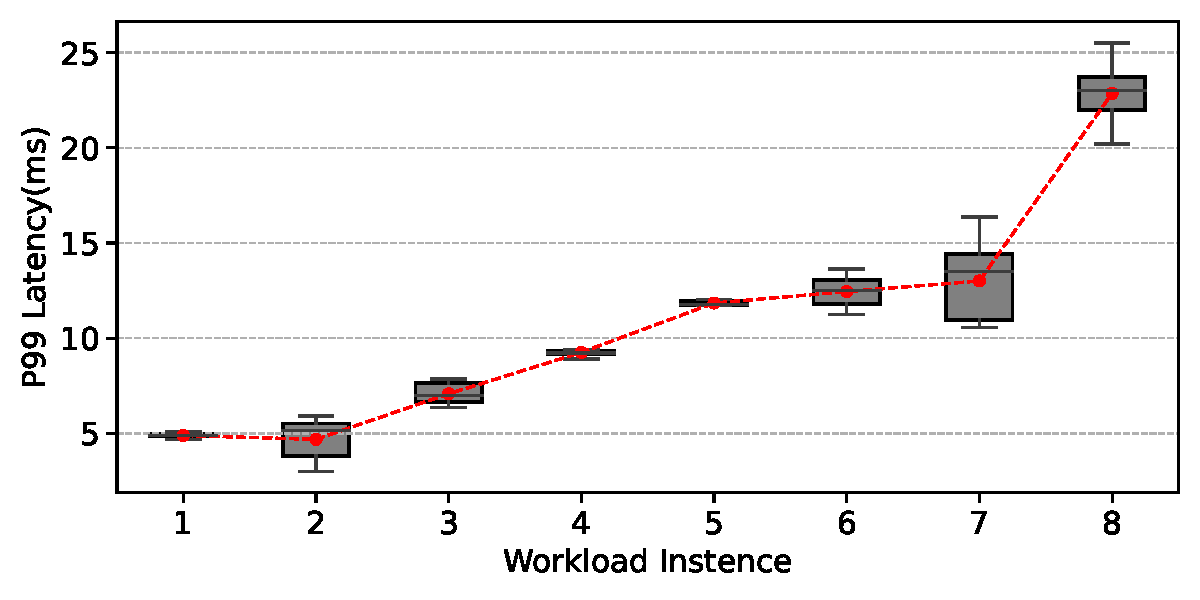
\includegraphics[width=\textwidth]{cpu_aware_box_eevdf_nice}
        \caption{混部场景EEVDF高优先级}
        \label{fig:cpu_aware_box_eevdf_nice}
    \end{subfigure}
\bicaption{\quad LC应用延迟稳定性}{\quad LC Application Latency Stability}
\label{fig:lc_box}
\end{figure}

同时从图~\ref{fig:lc_box}中能够看出,在BPF调度器下,LC应用的延迟稳定性也得到了一定的保障,这一方面是因为BPF调度器中的任务队列隔离机制,使得高优先级的LC应用总是能够被优先调度,另一方面则是因为BPF调度器没有信息墙,能够直接接触并调度任务,这是因为BPF调度器运行在内核中并遵循Core调度框架。

% \subsection{网络资源感知策略}

% \subsection{内存资源感知策略}
% Redis

\section{本章小结}

本章主要首先针对画像分析中不同类型应用,基于内核中关于HZ与抢占模型的配置,设计了调度配置的定制优化,提供了吞吐量优先与响应度优先两种不同调度目标的内核配置。

随后设计了混部场景下高优先应用与低优先级应用基于BPF调度策略的QoS保障机制,首先,提出了较为粗粒度的BPF调度队列隔离策略,利用调度类的优先级特性,使得在单个CPU上,低优先级能够感知高优先级任务的执行并出让CPU资源,从而保障高优先级应用的执行。

其次,基于BPF调度队列隔离策略,结合eBPF对于CPU与网络资源的感知实现更灵活的BPF资源感知调度策略,一方面相较于静态的CPU亲和性配置,CPU资源感知的调度策略能够动态地利用高优先级任务没有用到的核心,另一方面利用eBPF程序之间的交互性,能够方便地将其他子系统中的监测信息传递给BPF Scheduler进行辅助决策。

最后,比较了不同内核下的应用性能,说明对于不同的应用而言,定制的内核能够在一定程度上提升其运行性能。最后,通过不同应用,不同硬件环境下的混部实验,说明了使用BPF Scheduler来针对不同的混部场景进行定制优化,在提升高优先级应用的性能保障效果上的优势。